\documentclass[%
	corpo=11pt,
    twoside,
    stile=classica,
    oldstyle,
    tipotesi=custom,
    greek,
    evenboxes,
]{toptesi}
%%%%%%%%%%%%%%%%%%%%%%%%%%%%%%%%%%%%%%%%%%%%%%%%%%%%

\usepackage{listings}
\lstset{language=Matlab,%
      basicstyle=\small\ttfamily,
      numbers=left,
      numberstyle=\tiny,
      stepnumber=2,
      frame=lines
}

\usepackage[utf8]{inputenc}
\usepackage[T1]{fontenc}
\usepackage{lmodern}

\usepackage{hyperref}
\hypersetup{%
    pdfpagemode={UseOutlines},
    bookmarksopen,
    pdfstartview={FitH},
    colorlinks,
    linkcolor={blue},
    citecolor={blue},
    urlcolor={blue}
  }

%%%%%%% use PDFLATEX 

\usepackage{stix}
\usepackage{epigraph}

\usepackage{lipsum} %to insert random text

\usepackage{geometry} %for the margins
\newcommand\fillin[1][4cm]{\makebox[#1]{\dotfill}} %for the dotted line in the frontispiace

\usepackage{dcolumn}
\newcolumntype{d}{D{.}{.}{-1} } %to vetical align numbers in tables, along the decimal dot

\usepackage{amsmath}

\usepackage{natbib} % for the bibliography
\bibliographystyle{plainnat}


%%%%%%% Local definitions
\newtheorem{osservazione}{Osservazione}% Standard LaTeX
\newtheorem{observation}{Observation}% Standard LaTeX




%%%%%%%%%%%%%%%%%%%%%%%%%%%%%%%%%%%%%%%%%%%%%%%%
%%%%%%%%%%%%%%%%%%%%%%%%%%%%%%%%%%%%%%%%%%%%%%%%



\begin{document}\errorcontextlines=9
%\english

\begin{titlepage}
\newgeometry{left=1cm,right=1cm,top=3cm,bottom=3.5cm}  %specific margins for this page

\begin{center}

{\huge POLITECNICO DI TORINO}\\[1.5cm]
\textbf{Corso di Laurea\\in Matematica per l'Ingegneria}\\[3cm]
%\textbf{Corso di Laurea Magistrale\\in Ingegneria Matematica}\\[3cm]

{\Large Tesi di Laurea}\\[1cm]
%{\Large Tesi di Laurea Magistrale}\\[0.5cm]
\textbf{\LARGE Filtraggio di immagini }\\[2cm]

\includegraphics[width=0.2\textwidth]{./Pictures/logo_polito_2021.jpg}
\vspace{4cm}


\begin{minipage}{0.85\textwidth}
\begin{flushleft}\large
\textbf{Relatori} \hfill \textbf{Candidato}\\
prof. Nome Cognome \hfill Raffaello Ippolito\\
prof. Nome Cognome \\
\textit{firma dei relatori} \hfill \textit{firma del candidato}\\[0.35cm]
\fillin\ \hfill \\
\fillin\ \hfill \fillin
\end{flushleft}
\end{minipage}

\vfill

Anno Accademico 2021-2022
\end{center}

\restoregeometry %restor default margins 

\end{titlepage} %the frontispiece

%%%%%%% Dedication
\ifclassica%
{\begin{dedica}

    $\heartsuit$\ Alla mia regina
\end{dedica}
%%%%%%% 

\sommario%summary
%Here goes the abstrat of your thesis
Lo studio delle Equazioni alle derivate parziali ed il loro impiego in ambito di filtraggio di immagini.

%%%%%%%%%%%%%%%%%%%%%%%%%%%%%%%%%%%%%%%%%%%%%%%%
%%%%%%%%%%%%%%%%%%%%%%%%%%%%%%%%%%%%%%%%%%%%%%%%

\ringraziamenti%acknowledgements
%Acknowledge the people you love and/or work with
I candidati ringraziano vivamente il Granduca di Toscana per i mezzi messi loro a disposizione, ed il signor Von Braun, assistente del prof.~Albert Einstein, per le informazioni riservate che egli ha gentilmente fornito loro, e per le utili discussioni che hanno permesso ai candidati di evitare di riscoprire l'acqua calda.

%%%%%%%%%%%%%%%%%%%%%%%%%%%%%%%%%%%%%%%%%%%%%%%%
%%%%%%%%%%%%%%%%%%%%%%%%%%%%%%%%%%%%%%%%%%%%%%%%

\tablespagetrue\figurespagetrue%to include the list of tables
%and the list of figures - yuo can comment these commands

\indici%table of content
%It automatically generated

%%%%%%%%%%%%%%%%%%%%%%%%%%%%%%%%%%%%%%%%%%%%%%%%
%%%%%%%%%%%%%%%%%%%%%%%%%%%%%%%%%%%%%%%%%%%%%%%%

%Citation
%If you feel like a poetic guy!
\ifclassica   
\begin{citazioni}
    \textit{If you cannot understand my\\argument, and declare}\\
    it's Greek to me\\
    \textit{you are quoting Shakespeare.}
    
    [\textsc{B. Levin}, Quoting Shakespeare]\vspace{1em}
\end{citazioni}
\fi

%%%%%%%%%%%%%%%%%%%%%%%%%%%%%%%%%%%%%%%%%%%%%%%%
%%%%%%%%%%%%%%%%%%%%%%%%%%%%%%%%%%%%%%%%%%%%%%%%

\mainmatter

\part{Introduzione}
\chapter{Nozioni introduttive}

\section{Introduzione}
Le immagini hanno un ruolo fondamentale nelle nostre vite, viviamo di immagini, ne guardiamo tutti i giorni in tutti i contesti, la percezione visiva è sempre il nostro primo riferimento senza la quale ci si sentiamo persi.
Viviamo in una società consapevole di ciò e che sfrutta questo aspetto quanto più possibile nei campi più disparati, fotografie, radiografie, ecografie, poster pubblicitari, progetti, etc.
E' quindi un problema sempre di grande interesse cercare di sfruttarle al meglio, a tal fine esistono metodi cosìdetti di "filtraggio", tramite i quali intendiamo migliorare la qualità delle nostre immagini, mettere in risalto determinate caratteristiche o nasconderne altre.

Viviamo in un era digitale, le immagini passano generalmente per un calcolatore prima di essere stampate, o in ogni caso possono essere sempre scannerizzate (con strumenti più o meno precisi) così da averne una copia digitale.
E' in questa fase che l'immagine subisce il processo di filtraggio, nel calcolatore, quando pè in formato digitale, Per capire cos'è un filtro occorre dunque chiedersi cosa sia un'immagine digitale.

\section{Immagini digitali}
Per capire come codificare un'immagine per memorizzarla in fgormato digitale ci chiediamo prima che cos'è un'immagine.

\begin{quote}
\epigraph{Forma esteriore degli oggetti corporei, in quanto viene percepita attraverso il senso della vista, o si riflette – come realmente è, o variamente alterata – in uno specchio, nell’acqua e sim., o rimane impressa in una lastra o pellicola o carta fotografica.}{Vocabolario Treccani}
\end{quote}


Un'immagine viene rappresentata, impressa quindi su superfici, cioè oggetti bidimensionali, di dimensioni finite e le vediamo perchè i nostri occhi percepiscono il susseguirsi di colori diversi. Come codificare tali entità?
Come tutti gli oggetti reali, sebbene abbiano dimensioni finite, il susseguirsi delle immagini avviene in una maniera che possiamo considerare come continua. Questo è il primo problema che ci si pone quando si pensa a come codificare delle immagini.
La soluzione più largamente utilizzata è anche quella più semplice ed intuitiva, ossia di discretizzare tale distribuzione di colori. Dividiamo l'immagine con una griglia ed ad ogni casella, che d'ora in poi chiameremo "pixel", assegnamo un colore. 
E' ovvio che così facendo si perdono dei dettagli, la quantità di dettagli che riusciamo a conservare piò variare enormemente, un minimo si perde sempre ma è un  prezzo che siamo disposti a pagare.


Facciamo un esempio

%\ref{fig:figuraa}. 
\begin{figure}[htb] \centering
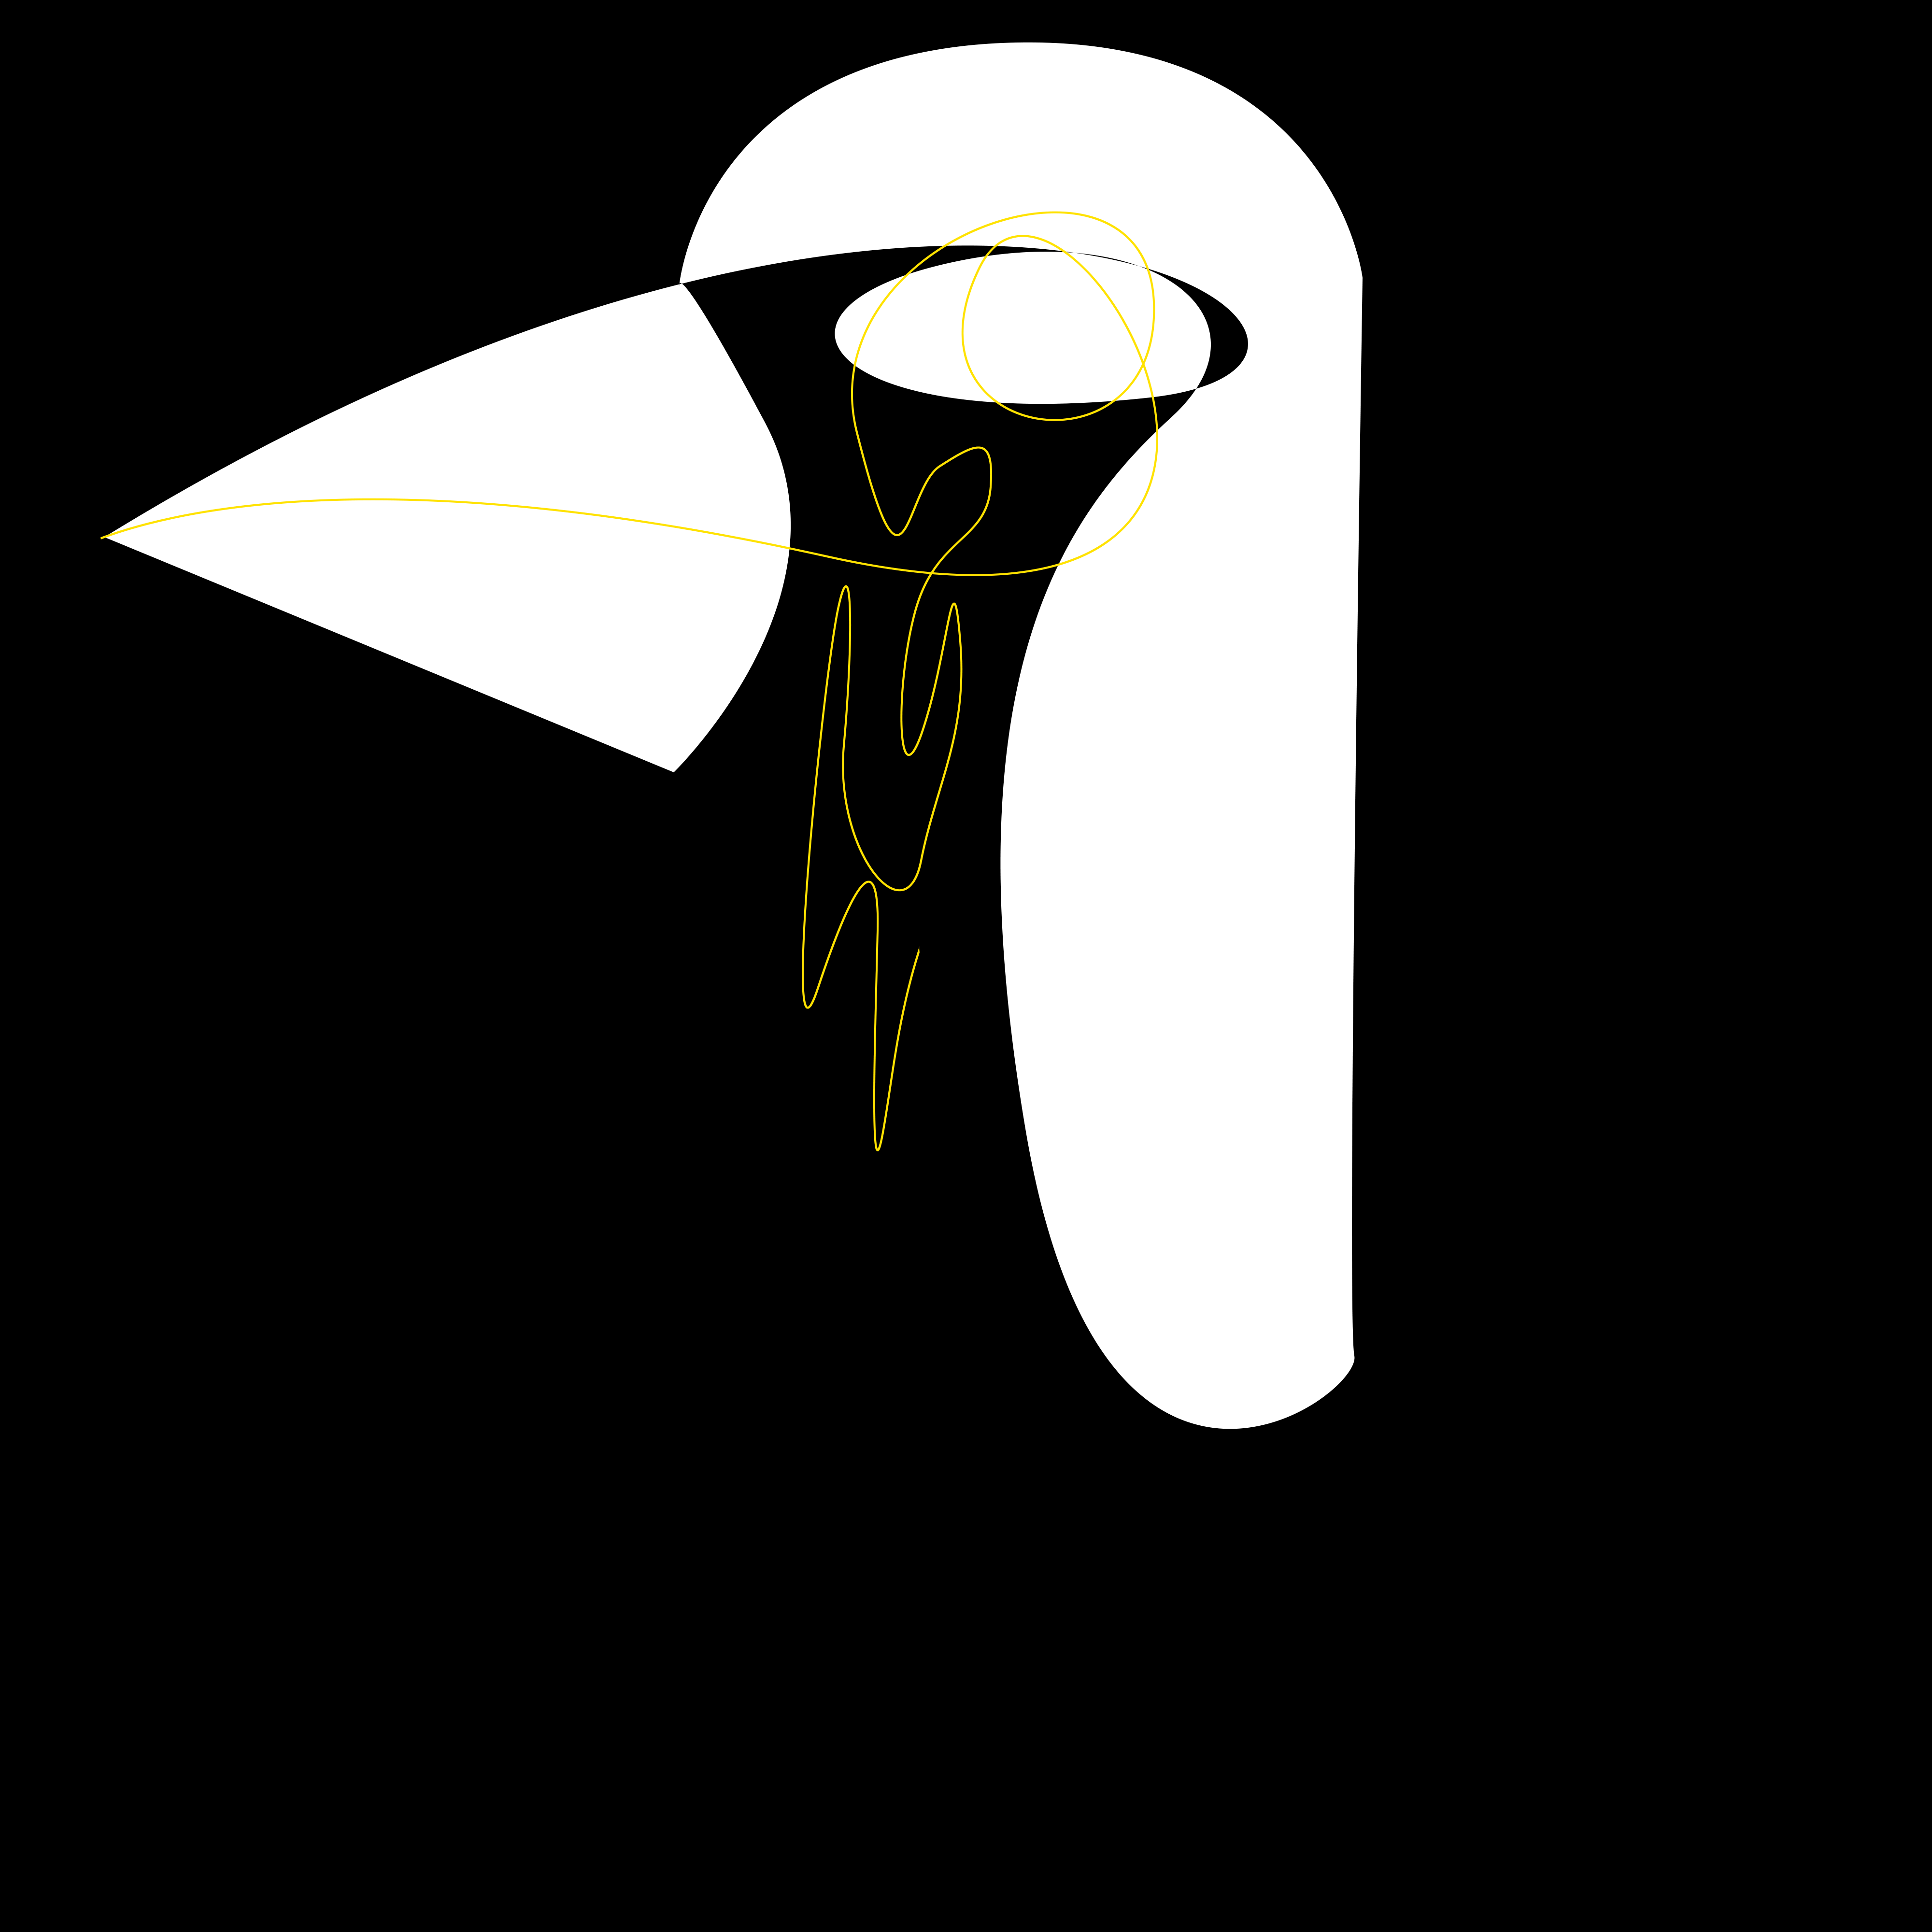
\includegraphics[scale=0.03]{Pictures/in ricordo del pinguino cameriere.png}
%\caption{Fiamme.}\label{fig:figura}
\qquad\qquad

\includegraphics[scale=0.03]{Pictures/canvas8x8.png}
\caption{Confronto immagine originale e immagine codificate utilizzando una griglia 4x4.}\label{fig:figura}
\end{figure}

%\ref{fig:figura}. 
\begin{figure}[htb] \centering
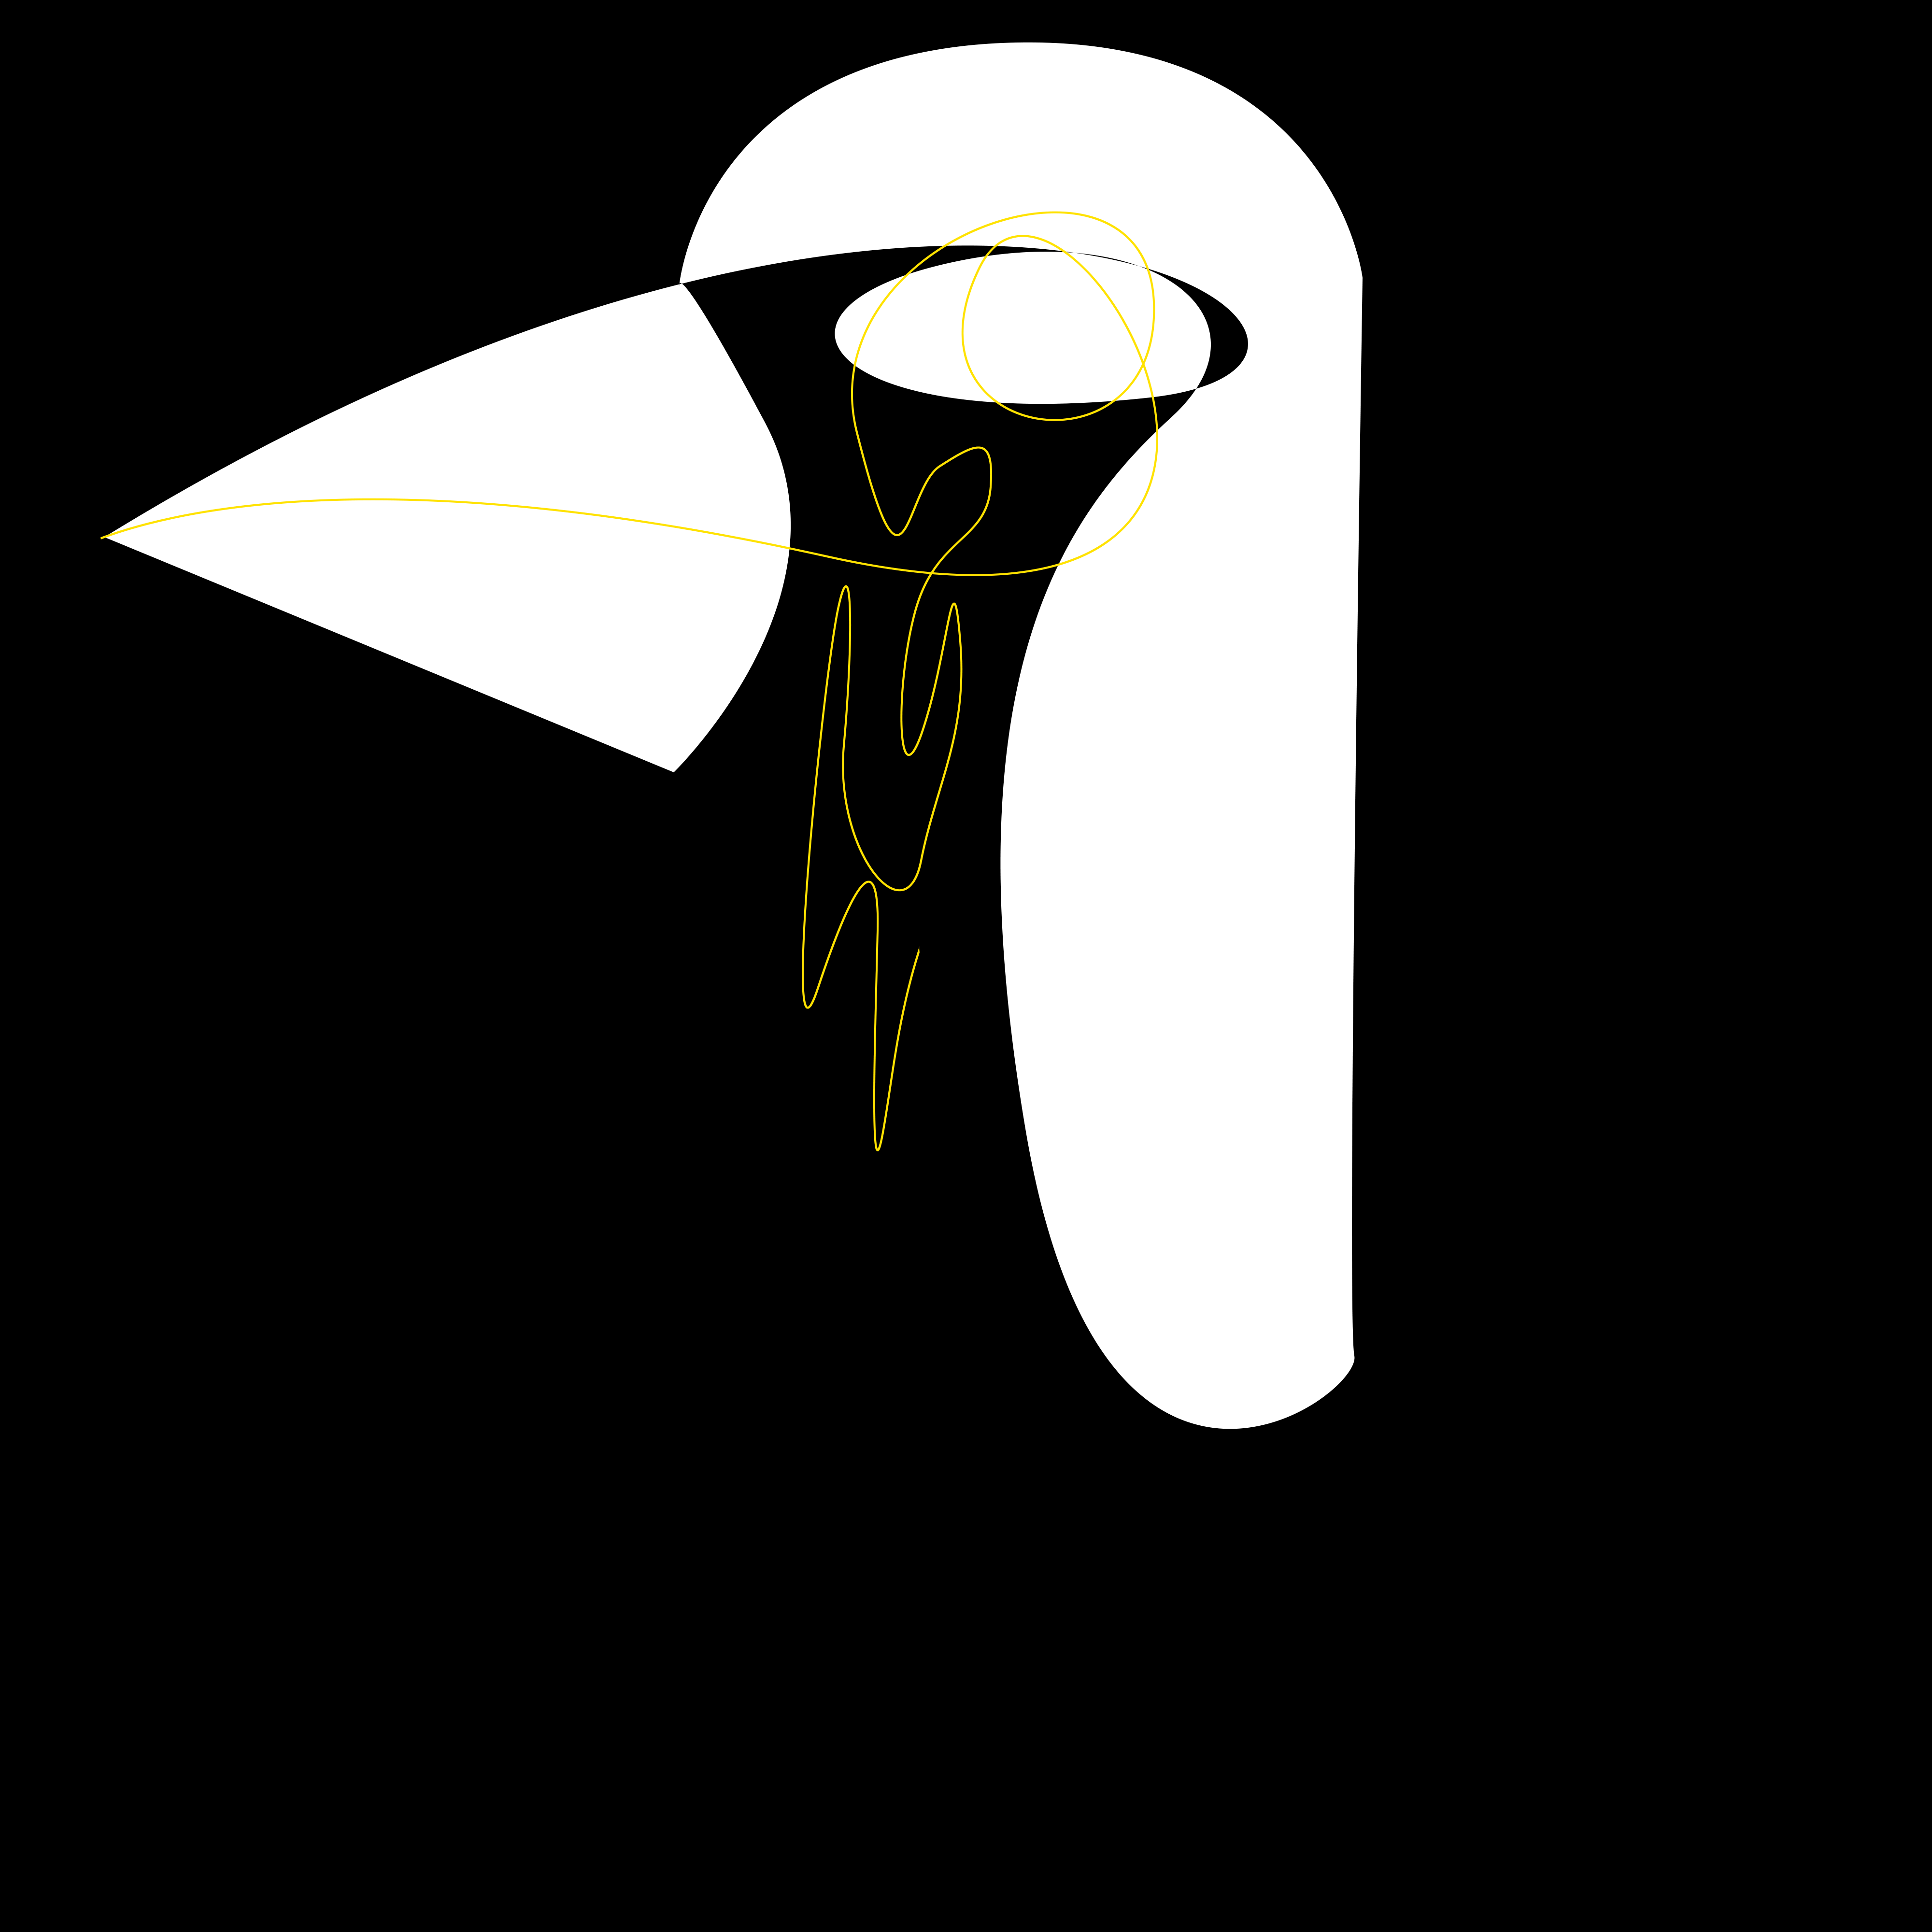
\includegraphics[scale=0.03]{Pictures/in ricordo del pinguino cameriere.png}
%\caption{Fiamme.}\label{fig:figura}
\qquad\qquad
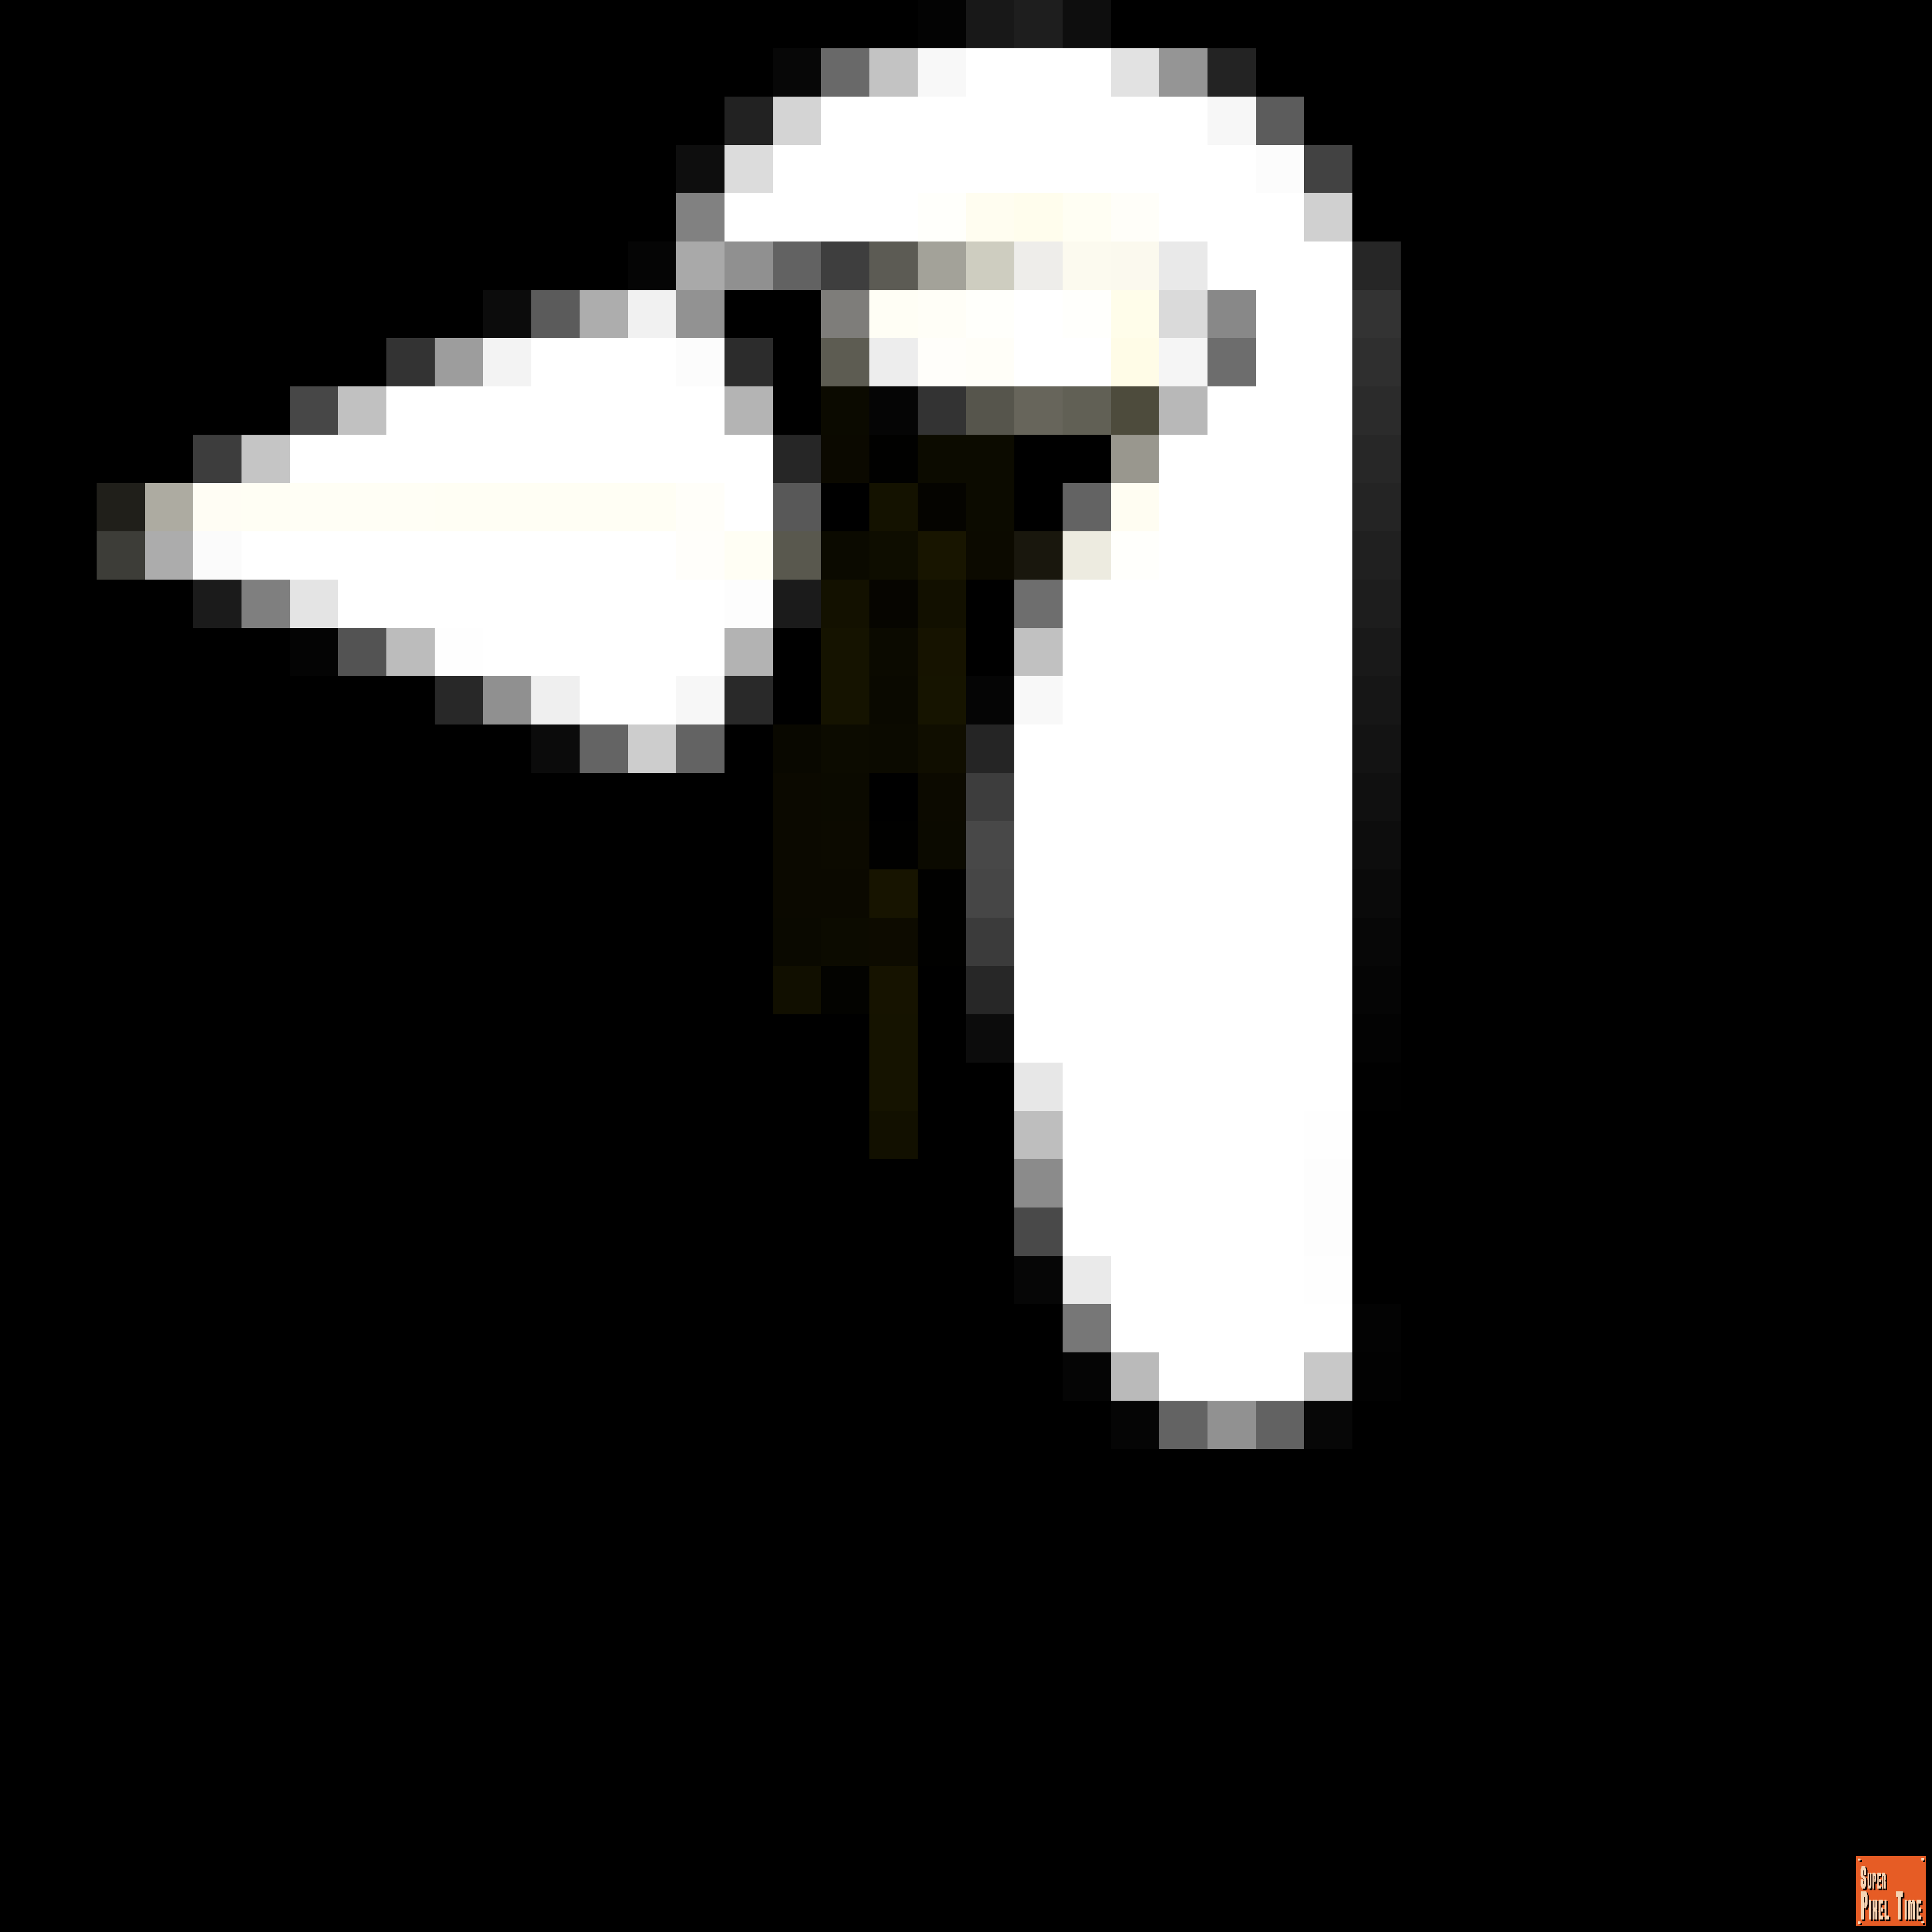
\includegraphics[scale=0.03]{Pictures/canvas80x80.png}
\caption{Confronto immagine originale e immagine codificate utilizzando una griglia 80x80.}\label{fig:figura}
\end{figure}

E' semplice vedere come ad una griglia più fitta corrisponda una miglior qualità dell'immagine, questo è il concetto di "risoluzione di un'immagine". 
Una miglior risoluzione però costa, come anticipato, in termini di memoria. Una griglia 4x4 corrisponde a 16 pixel, ad una griglia 80x80 corrispondono invece 6400 pixel! Questo vuol dire che la seconda immagine pesa 400 volte di più della prima.


Volendo definire in maniera più precisa cosa sia un'immagine digitale, diremmo che è una funzione da $\mathbb R^2$ in $\mathbb R^3$ siccome, date in input due cordinate questa funzione ci restituisce un colore (che è formato da 3 canali RGB).

\section{Cosa sono i filtri}
Una volta capito che un'immagine è una funzione possiamo definire un filtro come una seconda funzione che convoluta alla prima da il risultato richiesto.


Una equazione alle derivate parziali (PDE) esprime una evoluzione, sia u la nostra immagine e $u_0$ lo stato in cui si trova inzialmente, allora per convoluzione possiamo dire che 

\begin{equation} \label{eq:eq3}
u(x)=\frac{1}{w(x)}\int\int d(x-\xi)\Tilde{d}(u_0(x) -u_0(\xi))u_0(\xi)d\xi.
\end{equation}

\centering con  $w(x) = \int\int d(x-\xi)\Tilde{d}(u_0(x) -u_0(\xi))d\xi$\newline


\raggedright

Prendiamo in esame l'equazione del calore



\begin{equation} \label{eq:eq2}
\begin{cases}

\frac{\partial u}{\partial t}(t,x)-\Delta u(t,x) = 0 \ x \in \mathbb R^2, t\ge 0 \ .\\ 

u(0,x) = u_0(x)\ . \\

\end{cases}
\end{equation}
\part{Prima Parte}
\chapter{Equazione del calore e metodo Perna-Malik}

L'equazione del calore, come intuibile dal nome che porta, è stata formulata per determinare l'evoluzione di un sistema isolato che presenta al suo interno una data distribuzione di calore.\\

Euristicamente, non è difficile pensare che possiamo codificare (pensando ad un'immagine in bianco e nero) i pixel più luminosi come punti "più caldi" e quelli più scuri come punti "più freddi" ed applicare così l'equazione del calore.\\

vedremo con uno script MATLAB come opera nella pratica. \\
Per fare ciò opereremo una approssimazione alle differenze finite per il calcolo delle derivate.\\

\section{Metodo delle differenze finite}
Questo metodo, come anticipato, lo utilizzeremo per calcolare un valore approssimato delle derivate. Il proceimento si rifà molto alla definizione in se di derivata. Decidiamo quindi di approssimare \\
\vspace{2pt}
\centering 
$\frac{du}{dx} \approx \frac{u_{i+1} - u_i}{\Delta(x)} $\\
\vspace{2pt}
\raggedright
Se la derivata seconda è la derivata della derivata, allora approssimiamo \\
\vspace{3cm}
\centering                      
\begin{align*}
\frac{d^2u}{dx^2} \approx &
\frac{
(\frac{u_{i+1} - u_i}{\Delta(x)})_{i+1} 
- 
(\frac{u_{i+1} - u_i}{\Delta(x)})_i
}{\Delta(x)}
\\
\vline
\\
= &
\frac{
\frac{(u_{i+1} - u_i)_{i+1}}{\Delta(x)} 
-   
\frac{(u_{i+1} - u_i)_i}{\Delta(x)}
}{\Delta(x)}
\\
\vline 
\\
= &
\frac{
\frac{(u_{i+2} - u_{i+1})}{\Delta(x)} 
- 
\frac{(u_{i+1} - u_i)}{\Delta(x)}
}{\Delta(x)}
\\
\vline 
\\
= &
\frac{
\frac{(u_{i+2} - u_{i+1}) 
- 
(u_{i+1} - u_i)}{\Delta(x)}
}{\Delta(x)}
\\
\vline
\\
= &
\frac{
(u_{i+2} - u_{i+1}) 
- 
(u_{i+1} - u_i)}
{\Delta(x)^2}
\\
\vline 
\\
= &
\frac{
 u_{i+2} - u_{i+1} 
-u_{i+1} + {u_i}}
{\Delta(x)^2}
\\
\end{align*}

\raggedright
Per una migliore approssimazione è bene utilizzare un valore di $\Delta(x)$ quanto più basso possibile. Il massimo che possiamo fare è vedere la differenza tra un pixel e quello adiacente ossia $\Delta(x)=1$, ma allora 
$$\frac{d^2u}{dx^2} \approx
\frac{
 u_{i+2} - u_{i+1} 
-u_{i+1} + u_i}
{\Delta(x)^2} = u_{i+2} -2 u_{i+1} + u_i$$
Capiamo che scorrendo tutti gli indici questo è equivalente a $u_{i+1} -2 u_i + u_{i-1}.$

In sintesi utilizzeremo per il calcolo del laplaciamo l'approssimazione \\
\vspace{2pt}
\centering 
$\frac{d^2u}{dx^2} \approx u_{i+1} -2 u_i + u_{i-1}$\\
\vspace{2pt}
\raggedright

\section{Errore di troncamento}

Vale la pena di fare qualche considerazione sull'errore di troncamento che commettiamo adottando queste approssimazioni.\\
Per definizione, l'errore è la differenza tra il valore esatto e quello approssimato, ossia: 

$$
\frac{d^2u}{dx^2}\vline_{x_i}-\frac{u_{i+1}-u_i}{\Delta(x)}\approx \frac{\Delta(x)^2}{2} \frac{d^2u}{dx^2}\vline_\xi
$$

Risulta quindi evidente che l'errore dipende da $\Delta(x)^2$. 
Ad un'attenta analisi possiamo vedere che tra i metodi di approssimazione in avanti, in indietro o centrale, i primi due sono uguali tra di loro, quello centrale invece è diverso, esso dipende da un $\delta(x)^3$ e non da un $\delta(x)^2$, questo vuol dire che per $\delta(x)<1$ funziona meglio, per $\delta(x)>1$ funziona peggio. nel nostro caso $\delta(x)=1$ quindi la scelta è indifferente.
Ma procediamo con ordine.\\

Per brevità di notazione poniamo $\Delta(x)=h$.\\
Dagli sviluppi di Taylor in $x_j$ di
$u(x_{j \pm 1}) = u(x_j \pm h)$ fino al terzo ordine, si ottiene che

$$
u''(x_j) =\frac{u(x_{j+1}) - 2u(x_j) + u(x_{j-1})}{h^2} -\frac{1}{12} u(4)(\xi_j)h^2
$$

dove $\xi_j$ e un punto opportuno in $(x_{j-1} , x{j+1})$. Quindi, considerando il problema modello con condizoni di Dirichlet, per $j = 1,...,N-1$, si può scrivere che

$$
\frac{-u(x_{j+1}) + 2u(x_j) -u(x{j-1})}{h^2}
 + \frac{1}{12} u(4)(\xi_j)h^2 + \sigma(x_j)u(x_j) = f(x_j) .
$$

Se introduciamo la notazione $\tau_{j}=\frac{1}{12} u(4)(\xi_j)h^2$ (errore di troncamento locale) e poniamo:\\

$\boldsymbol{u}=[u_x...u_{N-1}]^T$\\
$\boldsymbol{\tau_h}=[\tau_x...\tau_{N-1}]^T$\\
$\boldsymbol{b_h}=[(f(x_1) + \frac{g_0}{h^2},f(x_2),...,f(x_{N-2}),f(x_{N-1}) + \frac{g_1}{h^2}]^T$\\

possiamo allora scrivere in forma matriciale,
$A_h\boldsymbol{u} = \boldsymbol{b_h} + \boldsymbol{\tau_h}$
dove $A_h = \frac{1}{h^2}
 tridiag(-1,2,-1) + diag(\sigma_1, ... ,\sigma_{N-1}) e \sigma_j = \sigma(x_j)$.\\
\vspace{1em}
Il metodo alle differenze finite consiste allora nel determinare un’approssimazione $u_h$ di
u andando a risolvere il sistema lineare
$A_hu_h = b_h.$
Osserviamo che $\boldsymbol{u_h}$ risulta ben definito in quanto $A_h$ è una matrice non singolare.\\

\vspace{1em}

Risultando che $\tau_h$ tende a zero quando h tende a zero, il metodo dicesi consistente. In particolare nel nostro caso, come osservato in partenza, risulta $\tau_h = O(h^2)$ .\\
Tuttavia la consistenza non assicura da sola la convergenza del metodo.\\
Per studiarne laconvergenza dobbiamo considerare il comportamento dell’errore $\boldsymbol{e_h} = \boldsymbol{u_h} -\boldsymbol{u}$ quando h tende a zero. Dato che risulta $A_h\boldsymbol{e_h} = \boldsymbol{\tau_h}$, e quindi $\boldsymbol{e_h} = A_h^{-1} \boldsymbol{\tau_h}$ possiamo scrivere: $||\boldsymbol{e_h}||\geq ||A_h^{-1}|| |\boldsymbol{\tau_h}||$\\
Vogliamo allora far vedere che, lavorando in norma infinito, siamo in grado di trovare una costante che, per ogni $h$, maggiora $||A_h^{-1}||$. \\
A questo scopo osserviamo che si può dimostrare che sia $A_h$ che la matrice $A_{0h} = \frac{1}{h^2} tridiag(-1,2,-1)$ hanno inversa non negativa, e si ha: 

$$A_{0h}^{-1}-A{h}^{-1}=A_{0h}^{-1}(A_h-A_{0h})A_h^{-1}\geq0$$

Per le ipotesi su $\sigma$ questo implica $A_h^{-1}||\leq A_{0h}^{-1}||$
osserviamo che
$||A_{0h}^{-1}||=max_j(A_{0h}^{-1}\boldsymbol{e})_j$ dove $\boldsymbol{e}$ indica il vettore di tutti 1.\\
Osservando che la soluzione esatta del problema $-u'' = 1, u(0) = u(1) = 0$, è il polinomio di secondo grado $\phi(x) = \frac{x(1-x)}{2}$, possiamo concludere che $A_{0h}^{-1}\boldsymbol{e})_j=\phi(x_j)$ e quindi che $A_h^{-1}||\leq A_{0h}^{-1}||\leq max_{0<x<1}|\phi_x|$.\\
Questo risultato di stabilità ci permette di concludere che l’errore $e_h$ ha lo stesso ordine dell’errore di troncamento $\boldsymbol{\tau_h}$ e di conseguenza che il metodo è convergente del secondo ordine.
Si noti che l’uniforme limitatezza della norma di $A_h^{-1}$ implica che il metodo numerico sia stabile 






\section{L'equazione del calore}

\raggedright

Prendiamo in esame l'equazione del calore

\begin{equation} 
\begin{cases}

\frac{\partial u}{\partial t}(t,x)-\Delta u(t,x) = 0 \ x \in \mathbb R^2, t\ge 0 \ .\\ 

u(0,x) = u_0(x)\ . \\

\end{cases}
\end{equation}

L'equazione del calore, come intuibile dal nome che porta, è stata formulata per determinare l'evoluzione di un sistema isolato che presenta al suo interno una data distribuzione di calore. E' banale pensare che con il passare del tempo il calore si distribuisca, tendendo per un tempo infinito ad una distribuzione uniforme.

\vspace{1em}

Euristicamente, non è difficile pensare che possiamo codificare (pensando ad un'immagine in bianco e nero) i pixel più luminosi come punti "più caldi" e quelli più scuri come punti "più freddi" ed applicare così l'equazione del calore.\\
Otteniamo quindi un'immagine sempre più "liscia", otteniamo di fatto una sfocatura, e per un numero di iterazioni idealmente infinito ci ritroveremmo con una distribuzione uniforme di colore, ossia una tinta unita.

\vspace{1em}

Vediamo con uno script matlab come opera nella pratica. \\

\begin{lstlisting}[language=MATLAB]
Im=imread('parrot.jpeg');   %Apro l'immmagine
Im=rgb2gray(Im);            %La trasformo in bianco e nero
Im = imnoise(Im,'gaussian');%Aggiungo del rumore

%---Definisco le costanti e le condizioni iniziali

[ny, nx, ~]=size(Im)        %Dimensioni dell'immagine
dt=0.25;                    %Passo temporale
u=double(Im);               %Copia dell'immagine originale su cui                                lavorare
T=3			                    %Tempo, ossia T/dt + 1 definisce il numero                            di iterazioni da eseguire
k=0.5;

%---Mostro l'immagine originale
imshow(uint8(Im))
title('immagine originale'); 

%---Metodo eq del calore
u=double(Im);
for t = 0:dt:T
   u_xx = u(:,[2:nx nx],:) - 2*u + u(:,[1 1:nx-1],:);  % derivata                                                           seconda lungo x
   u_yy = u([2:ny ny],:,:) - 2*u + u([1 1:ny-1],:,:);  % derivata                                                            seconda lungo y
   u= u + k*dt*(u_xx+u_yy);
   temp=u;
end

\end{lstlisting}
\vspace{1em}
Provando a cambiare il tempo, ossia il numero di iterazioni, osserviamo come un maggior lasso di tempo produca immagini più sfocate. \\

\begin{figure}[htb] 
\centering
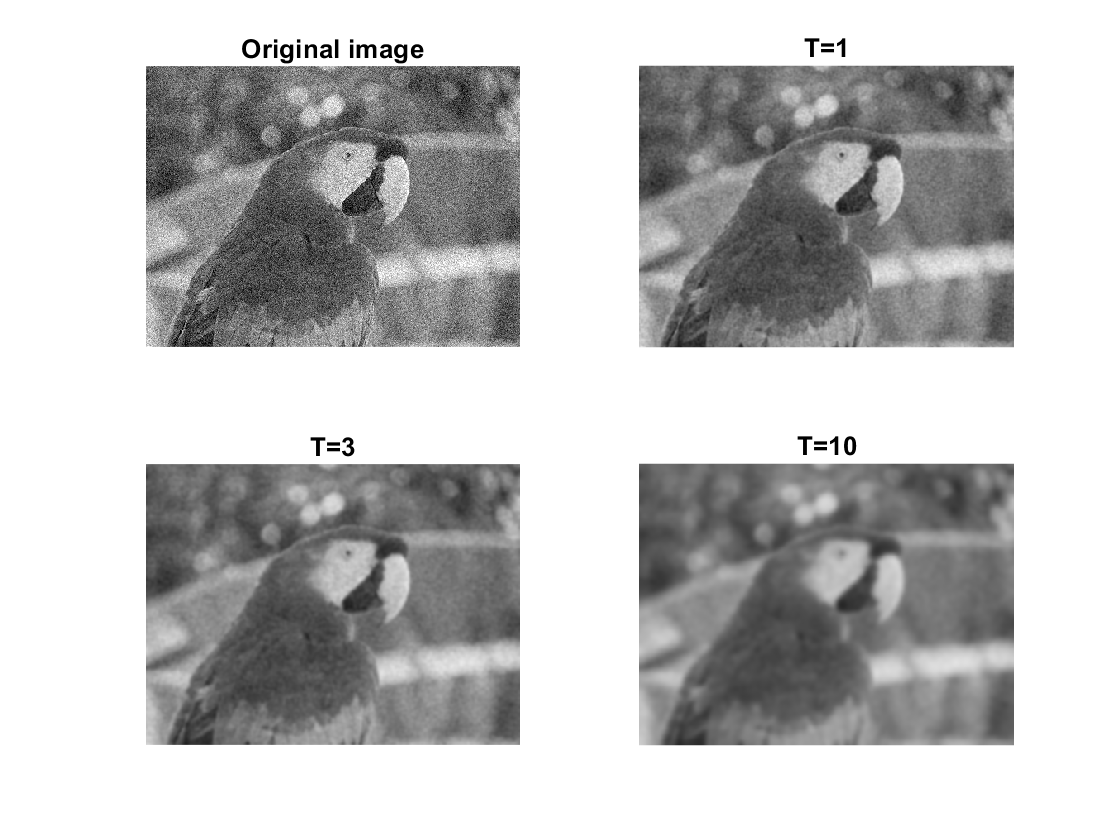
\includegraphics[scale=0.4]{Pictures/Risultati/eq del calore.png}
%\caption{Fiamme.}\label{fig:figura}
%\qquad\qquad
%
\includegraphics[scale=0.03]{Pictures/canvas8x8.png}
\caption{Effetti dell'eq del calore nel tempo.}\label{fig:figura}
\end{figure}


Questo metodo però non è poi molto utile in generale, sì, il rumore viene eliminato o almeno ridotto ma si perdono importanti dettagli, esistono procedimenti come il metodo Perona-Malik che sono decisamente più utili. L'idea del metodo Perona-Malik è di applicare l'equazione del calore nelle regioni in cui il colore è più uniforme, così da preservarne i bordi\\


\section{Rilevamento dei bordi}

Operando una derivata in una data direzione, per il significato in sè di derivata, questa assume valori più elevati quando la variazione è elevata, e assume valori nulli quando non c'è variazione in quella direzione. Per questo motivo, applicata ad un' immagine, ne rileviamo i bordi!\\
Presa una tinta unita la derivata sarà quindi nulla in ogni suo punto (è intuitivo, se un'immagine è una funzione che, date due coordinate restituisce un colore, allora una tinta unita è una funzione costante ed in quanto tale ha derivata nulla).\\
\vspace{1em}
Operando una derivata seconda in una data direzione, per il significato in sè di derivata seconda, questa assume valori più elevati quando la concavità è più stretta, e assume valori pressocchè nulli quando non ci sono concavità (possiamo pensare alle concavità come a dei picchi o dei ventri, su di una immagine vuol dire chiazze di colore diverso).\\
Presa una sfumatura di colore che varia in maniera lineare, la derivata seconda sarà nulla in ogni suo punto, la derivata prima sarà invece costante. 
Scriviamo un piccolo script su MATLAB che ci mostri questo aspetto

\begin{lstlisting}[language=MATLAB]
%---Operazioni preliminari
Im=imread("nome_immagine.png");	%Apro l'immmagine

[ny, nx, ~]=size(Im)        %Memorizzo le dimensioni dell'immagine
u=double(Im);               %Copia dell'immagine originale su cui lavorare
h=80;                       %Definisco un parametro che usero' per                               enfatizzare i bordi in fase di stampa 


%---Calcolo tutte le derivate
u_x =  u(:,[1 1:nx-1],:) - u;                       %derivata                                                            prima lungo x
u_xx = u(:,[2:nx nx],:) - 2*u + u(:,[1 1:nx-1],:);  %derivata                                                            seconda lungo x
u_y =  u([1 1:ny-1],:,:) - u;                       %derivata                                                            prima lungo y
u_yy = u([2:ny ny],:,:) - 2*u + u([1 1:ny-1],:,:);  %derivata                                                            seconda lungo y
u_xy = u_x([1 1:ny-1],:,:) - u_x;                   %derivata                                                            seconda mista
   
%---Stampo i risultati
figure()
subplot(2,3,2),text(0.3,0,nome,'FontSize',20); axis off
subplot(2,3,4), imshow(Im)
title('Immagine originale')
subplot(2,3,5), imshow(uint8(h*abs(u_x)))
title('h*u_x')
subplot(2,3,6), imshow(uint8(h*abs(u_y)))
title('h*u_y')

figure()
subplot(2,3,2),text(0.3,0,nome,'FontSize',20); axis off
subplot(2,3,4), imshow(Im)
title('Immagine originale')
subplot(2,3,5), imshow(uint8(h*abs(u_x + u_y)))
title('h*(u_x + u_y)')
subplot(2,3,6), imshow(uint8(h*abs(u_xx + u_yy)))
title('h*(u_xx + u_yy)')
\end{lstlisting}

\vspace{6em}
Vediamo con diverse immagini molto semplici se otteniamo i risultati attesi.\\
%\vspace{1em}

\begin{figure}[htb] 
\centering
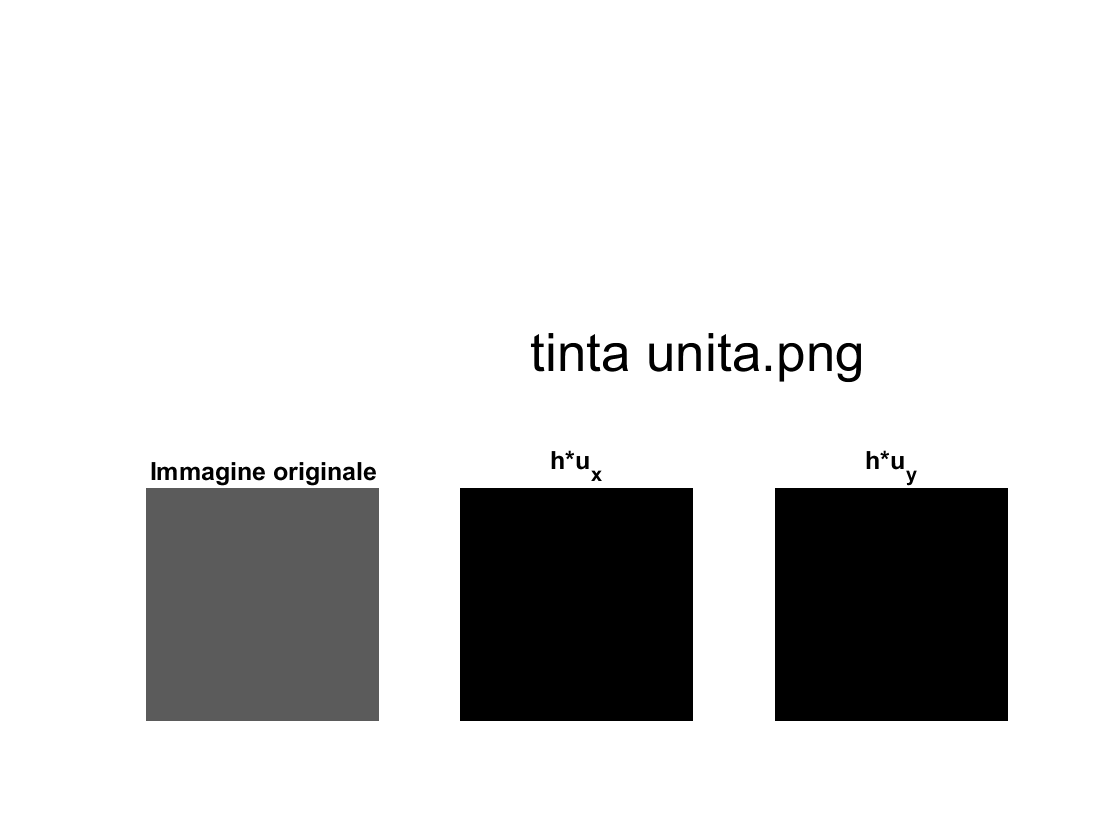
\includegraphics[scale=0.4, trim = 0 0 0 10.5cm, clip]{Pictures/Risultati/tinta unita bianco e nero derivate parziali.png}
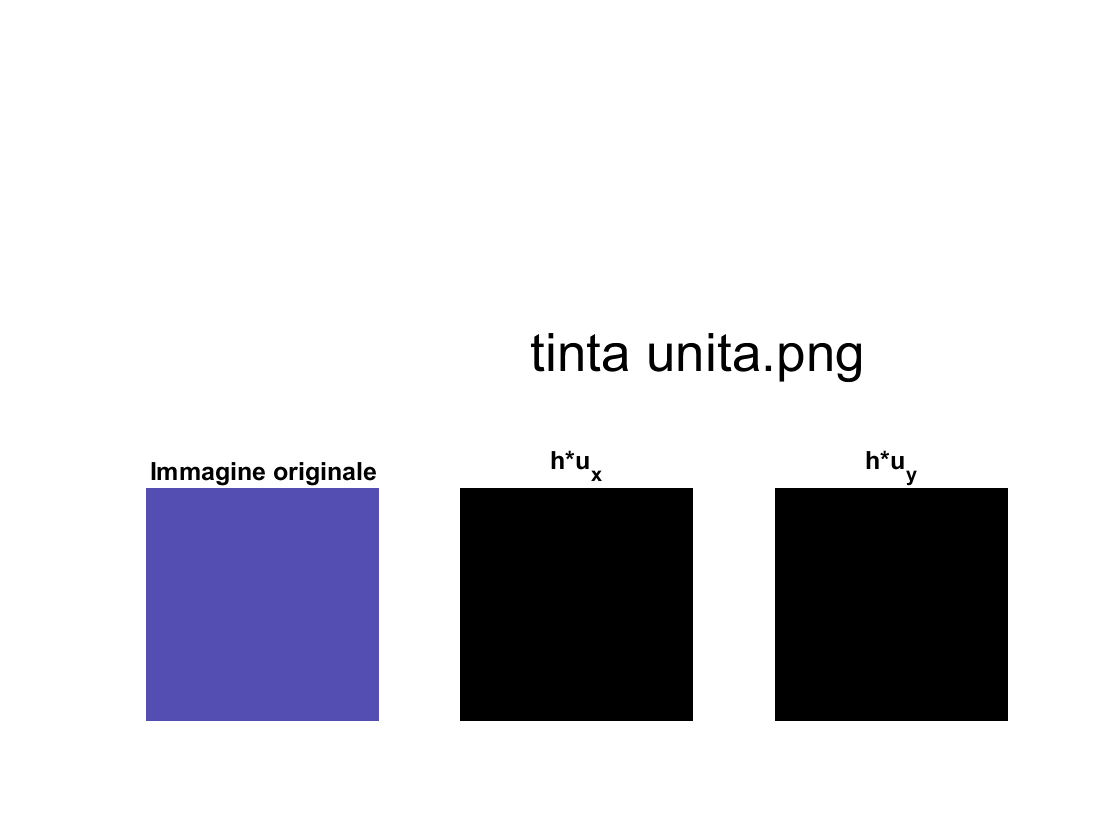
\includegraphics[scale=0.4, trim = 0 0 0 10.5cm, clip]{Pictures/Risultati/tinta unita derivate parziali.png}
\caption{Derivate parxiali di una tinta unita.}\label{fig:figura}
\end{figure}

Possiamo vedere come con un'immagine a tinta unita (che sia essa in bianco e nero o a colori) le derivate sono nulle, quindi lo saranno anche gradiente e laplaciano. Confermiamo inoltre che questi principi valgono sia a colori che in bianco e nero.\\

\newpage
\begin{figure}[htb] 
\centering
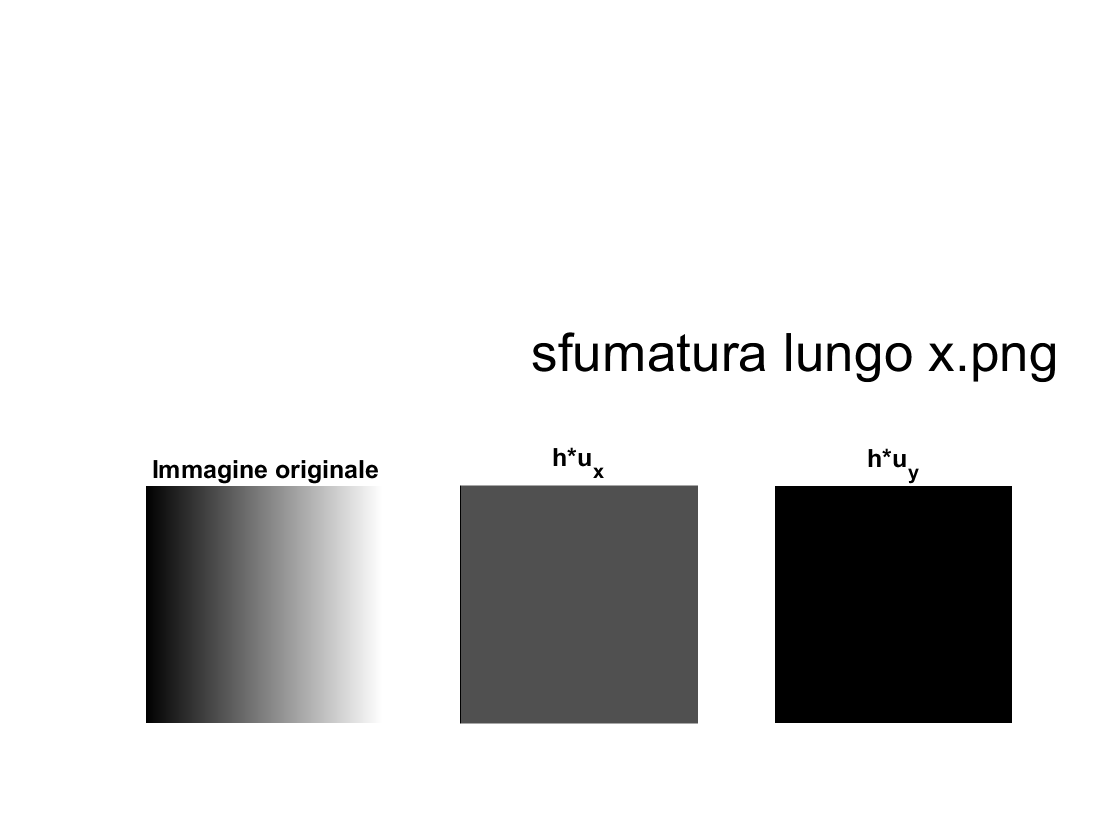
\includegraphics[scale=0.4, trim = 0 0 0 10.5cm, clip]{Pictures/Risultati/sfumatura lungo x bianco e nero derivate parziali.png}
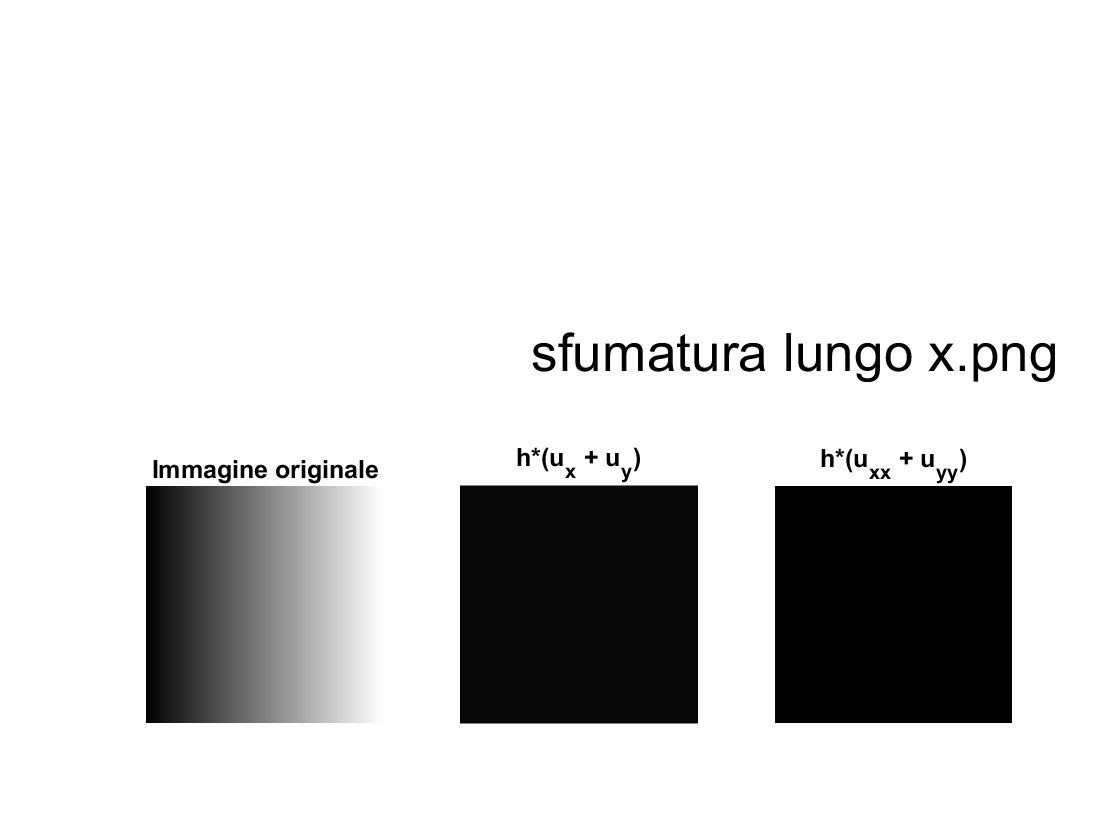
\includegraphics[scale=0.4, trim = 0 0 0 10.5cm, clip]{Pictures/Risultati/sfumatura lungo x bianco e nero gradiente e laplaciano.png}
\caption{Derivate parziali, gradiente e laplaciano di una sfumatura orizzontale.}\label{fig:figura}
\end{figure}

Guardando invece ad una immagine che presenta una sfumatura lineare lungo l'asse x, la derivata lungo x assume un valore costante mentre la derivata lungo y è nulla, proprio perchè lungo y non c'è variazione mentre lungo x c'è una variazione costante.\\
Ovviamente, date queste premesse, il gradiente sarà costante uguale $u_x$ (siccome $u_y=0$) e quindi il laplaciano sarà nullo.
Il fatto che in entrambi questi esempi il laplaciano sia nullo è un buon segno, lo useremo per rilevare i bordi ed in queste immagini non ve ne sono, quindi è giusto che il laplaciano sia nullo.\\

\newpage
\begin{figure}   
\centering
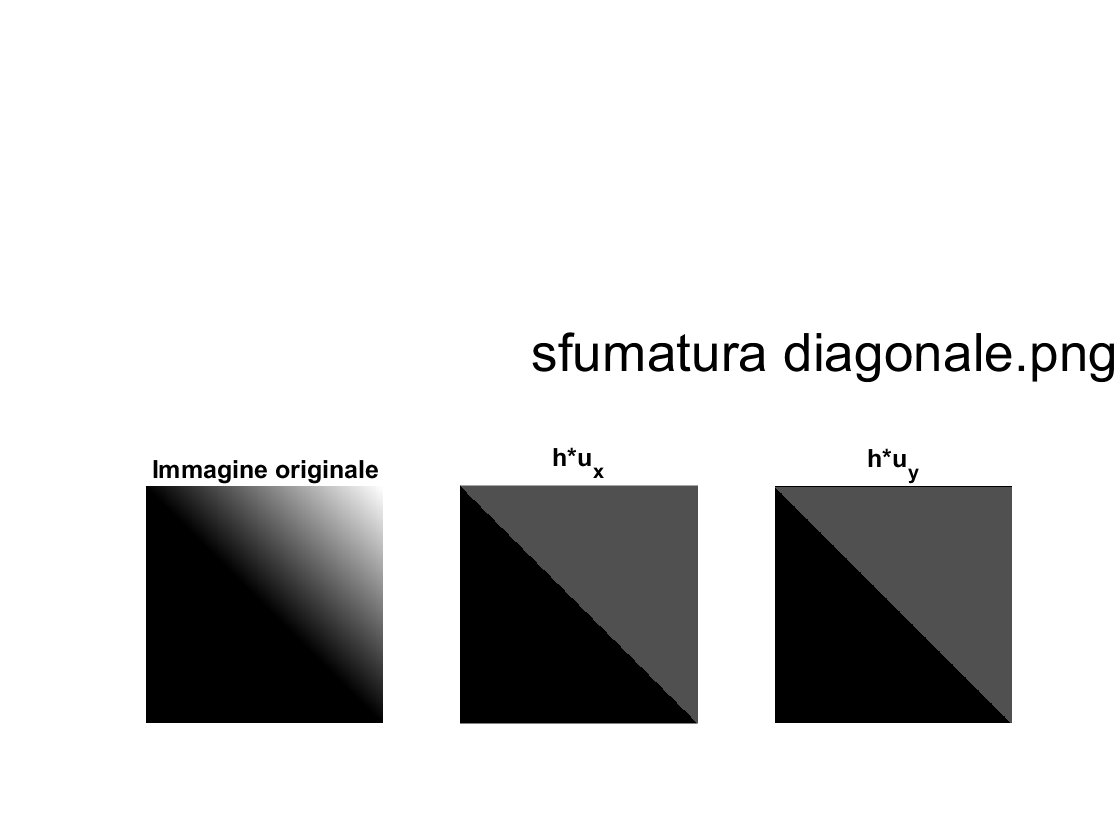
\includegraphics[scale=0.4, trim = 0 0 0 10.5cm, clip]{Pictures/Risultati/sfumatura diagonale bianco e nero derivate parziali.png}
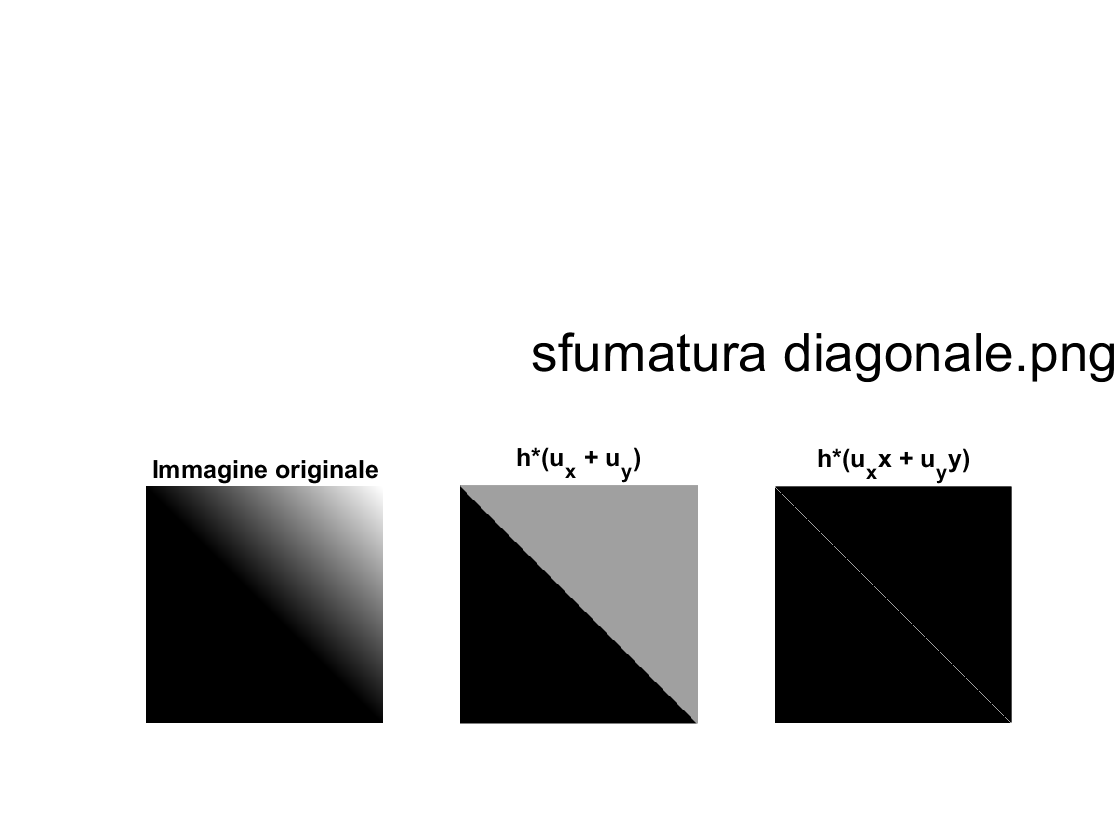
\includegraphics[scale=0.4, trim = 0 0 0 10.5cm, clip]{Pictures/Risultati/sfumatura diagonale bianco e nero gradiente e laplaciano.png}
\caption{Derivate parziali, gradiente e laplaciano di una sfumatura diagonale.}\label{fig:figura}
\end{figure}

Se prendiamo una sfumatura diagonale ma solo su metà immagine vediamo dei riultati interessanti: entrambe le derivate parziali sono nulle nelle regioni in cui non c'è sfumatura, esattamente come nel caso della tinta unita, ed entrambe sono costanti dove c'è sfumatura (che ricordiamo essere lineare).\\
Tutto ciò riconferma quanto visto dai punti precedenti, decidiamo quindi di volgere uno sguardo al gradiente ed al laplaciano e noteremo qualcosa di interessante, il gradiente ha un aspetto molto simile alle due derivate parziali, sommando i loro valori è semplicemente più luminoso.\\
Per quanto riguarda il gradiente la storia cambia. Le derivate seconde sono indicatrici della variazione delle derivate prime, cioè della variazione della variazione del valore della funzione, ma l'unica variazione che hanno le derivate prime è lungo la diagonale.
Abbiamo così individuato il nostro primo bordo, cioè la diagonale che divide di fatto due regioni, una in cui il colore è costante ed una in cui sfuma.\\

\vspace{1em}

Facciamo ancora un esempio, proviamo ad introdurre una semplice figura e vediamo cosa accade.\\

\newpage
\begin{figure}[htb] 
\centering
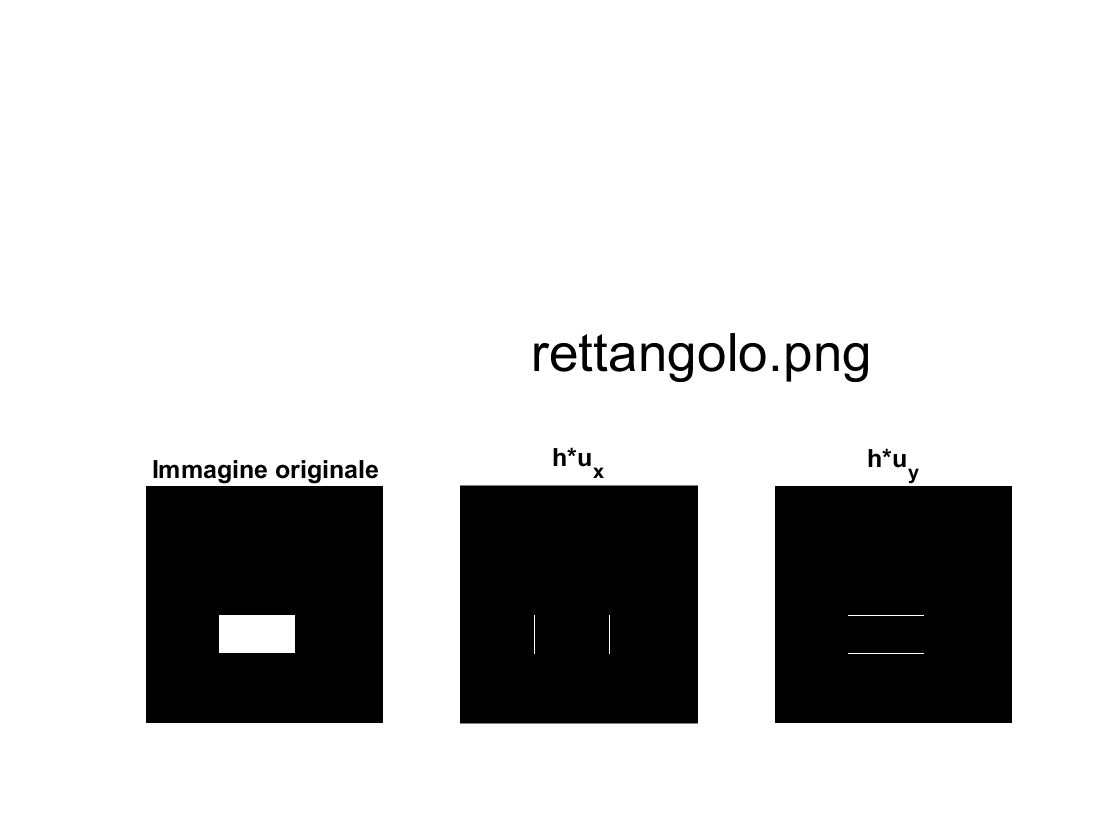
\includegraphics[scale=0.4, trim = 0 0 0 10.5cm, clip]{Pictures/Risultati/rettangolo bianco e nero derivate parziali.png}
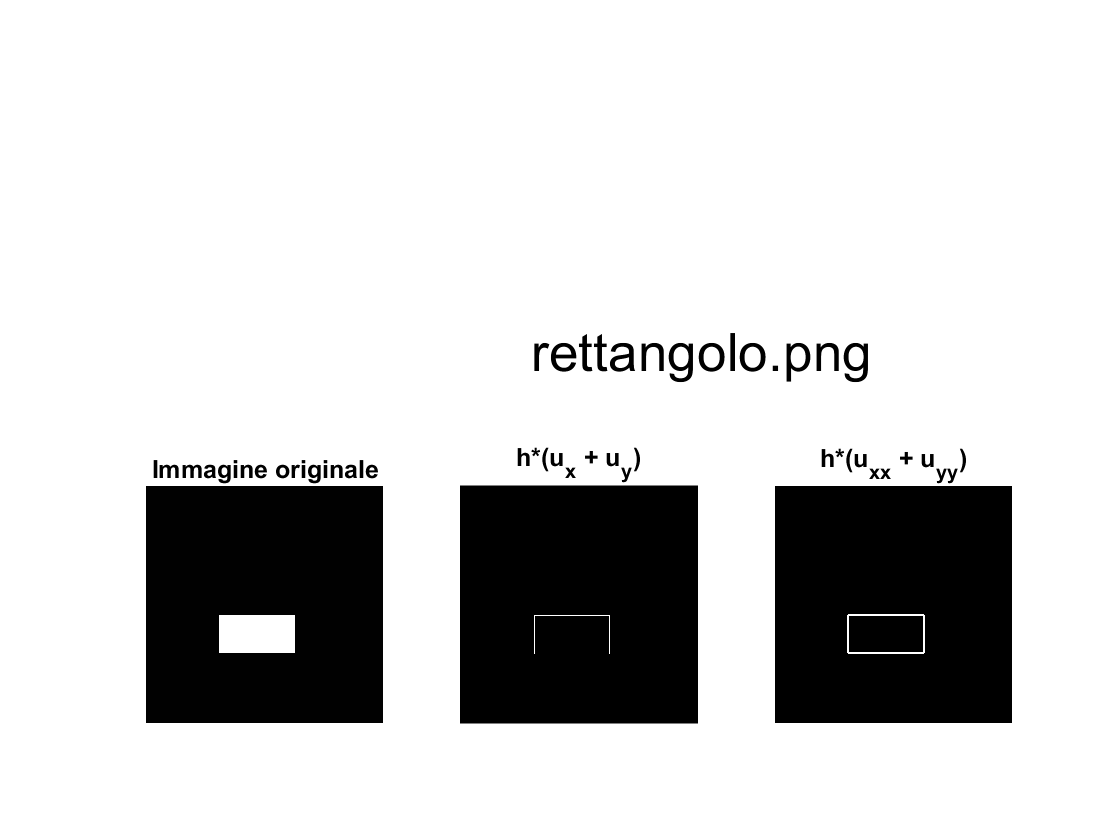
\includegraphics[scale=0.4, trim = 0 0 0 10.5cm, clip]{Pictures/Risultati/rettangolo bianco e nero gradiente e laplaciano.png}
\caption{Derivate parziali, gradiente e laplaciano di una figura semplice.}\label{fig:figura}
\end{figure}

Abbiamo importato un rettangolo nero su di uno sfondo bianco, come confermato anche dalla prima sfumatura, la derivata lungo x rileva i bordi verticali, quella lungo y i bordi orizzontali, dalla loro somma (quindi dal gradiente) otteniamo già il bordo del rettangolo.
Il bordo così ottenuto è un bordo che idealmente rimarrà inalterato a prescindere dall'ordine della derivata, in particolare quindi anche per derivate seconde, quindi il laplaciano continua a soddisfare la nostra richiesta di determinare i bordi. \\
Come detto: "Il bordo così ottenuto è un bordo che idealmente rimarrà inalterato a prescindere dall'ordine della derivata" cerchiamo di capire perchè. Presa una striscia di pixel, cioè uno strato della nostra immagine (immaginiamola quindi come una funzione da R in R), otterremo quindi una funzione porta!\\
La funzione porta non è derivabile in senso classico, ripensando alla definizione di derivata avremmo un valore di +infinito prima e -infinito poi. La sua derivata sarà quindi una coppia di delta di Dirac\\












\bibliography{references}



\end{document}

\